\documentclass[border=15pt, tikz]{standalone}
\usepackage[T1]{fontenc}
\usepackage[utf8]{inputenc}
\usepackage{tikz}
\usetikzlibrary{positioning, arrows.meta, decorations.pathreplacing, calc, fit}
\definecolor{clrattention}{HTML}{00B4D8}
\definecolor{clrattention_alt}{HTML}{90E0EF}
\definecolor{clrffn}{HTML}{E63946}
\definecolor{clrnorm}{HTML}{FFBE0B}
\definecolor{clrembed}{HTML}{06D6A0}
\definecolor{clrresidual}{HTML}{118AB2}
\definecolor{clroutput}{HTML}{7B2CBF}
\definecolor{clrspectral}{HTML}{00F5D4}
\definecolor{clrphysics}{HTML}{F77F00}
\definecolor{clrborder}{HTML}{073B4C}
\definecolor{clrtext}{HTML}{073B4C}
\definecolor{clrgroup_frame}{HTML}{073B4C}
\definecolor{clrgroup_fill}{HTML}{EDF6F9}
\begin{document}
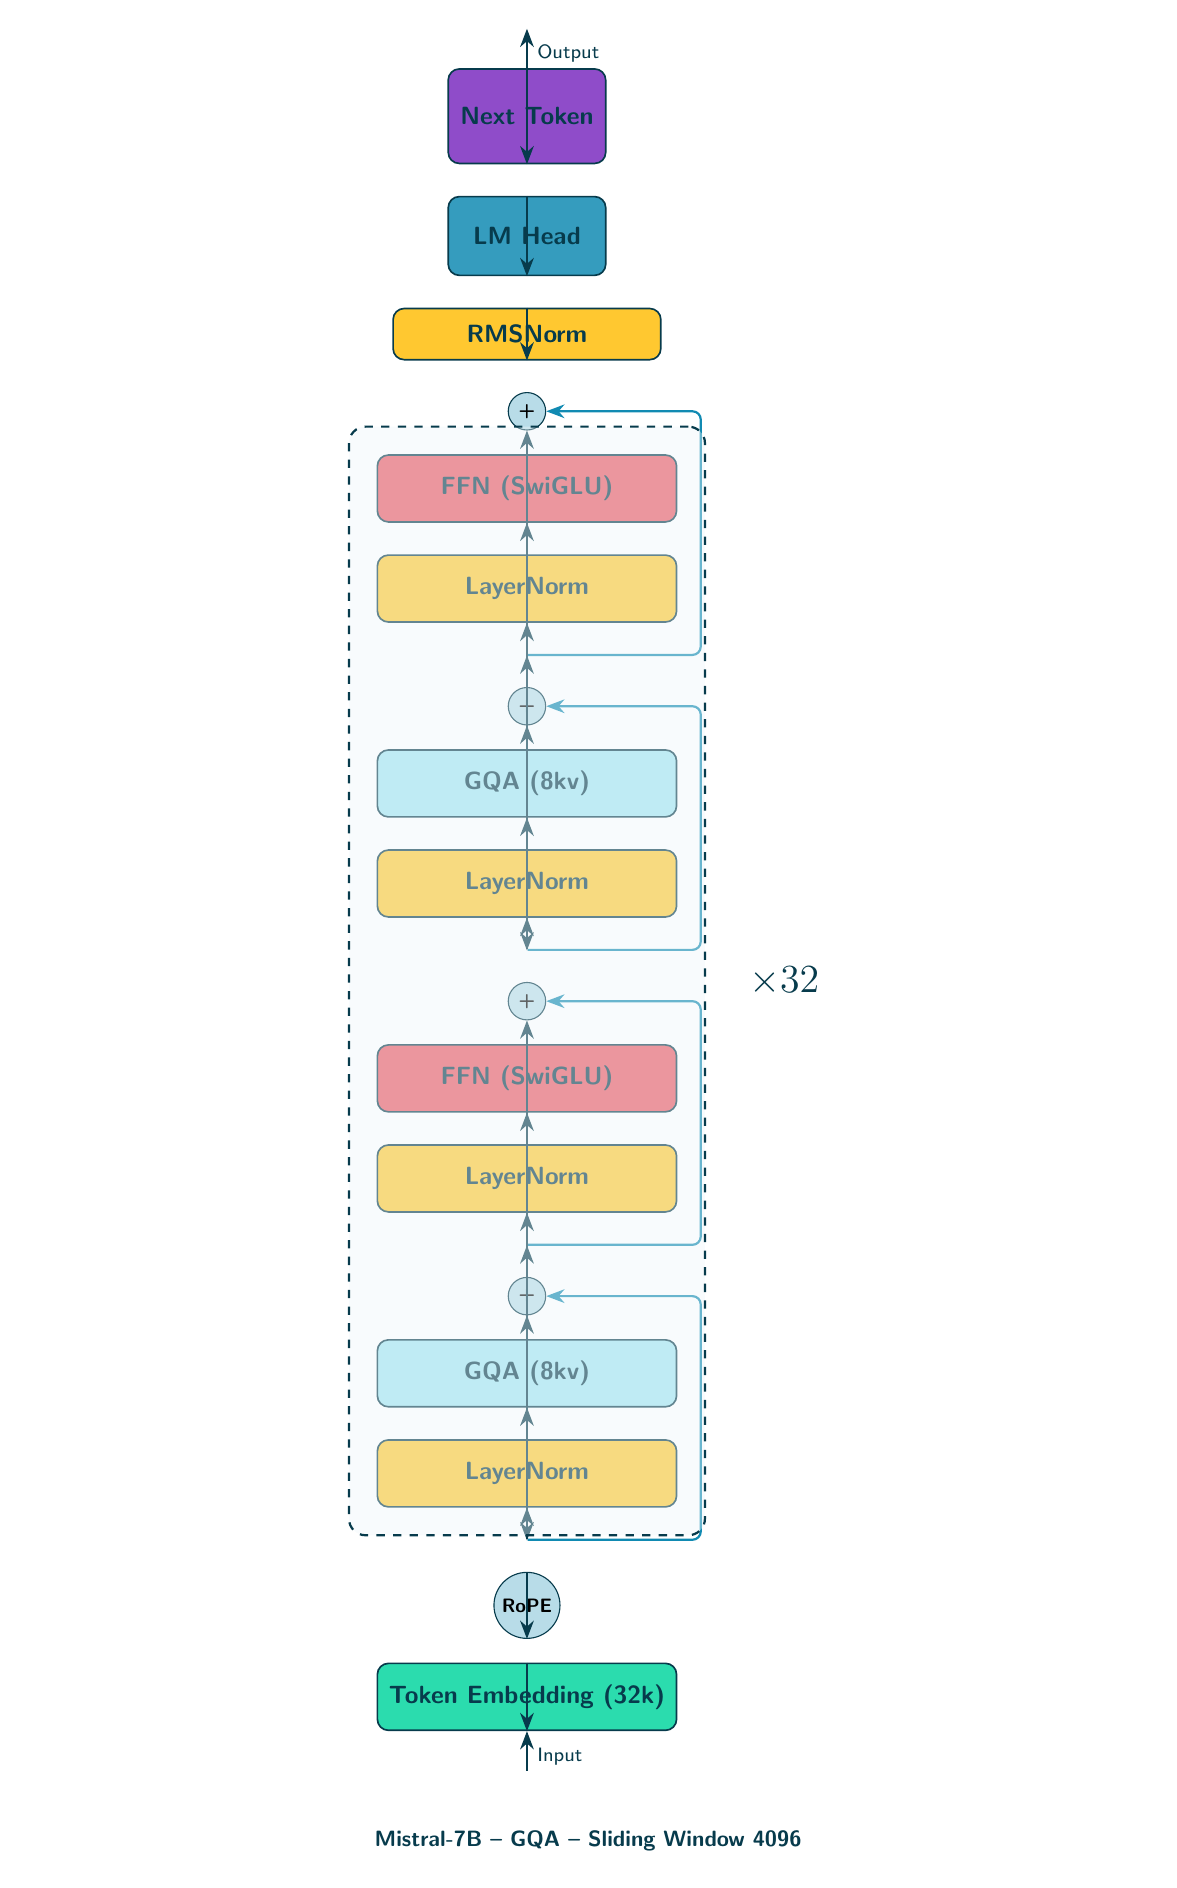
\begin{tikzpicture}[
    >=Stealth,
    every node/.style={font=\sffamily},
    block/.style={draw=clrborder, rounded corners=4pt, minimum width=3.8cm,
                  minimum height=0.85cm, font=\sffamily\small\bfseries,
                  text=clrtext, line width=0.6pt},
    arrow/.style={->, thick, color=clrborder, line width=0.8pt},
    skiparrow/.style={->, thick, color=clrresidual, line width=0.8pt, rounded corners=3pt},
    label/.style={font=\sffamily\scriptsize, text=clrtext},
    subtitle/.style={font=\sffamily\footnotesize, text=clrtext},
]
\node[block, fill=clrembed!85, minimum width=3.8cm, minimum height=0.85cm, text=clrtext] (n_1) at (0,0) {Token Embedding (32k)};
\node[circle, draw=clrborder, fill=clrresidual!30, inner sep=2pt, font=\sffamily\scriptsize\bfseries, above=0.3cm of n_1] (n_2) {RoPE};
\node[inner sep=0, minimum size=0, above=0.4cm of n_2] (res_entry_3) {};
\node[block, fill=clrnorm!85, minimum width=3.8cm, minimum height=0.85cm, text=clrtext, above=0.4cm of res_entry_3] (n_4) {LayerNorm};
\node[block, fill=clrattention_alt!85, minimum width=3.8cm, minimum height=0.85cm, text=clrtext, above=0.4cm of n_4] (n_5) {GQA (8kv)};
\node[circle, draw=clrborder, fill=clrresidual!30, inner sep=2pt, font=\sffamily\scriptsize\bfseries, above=0.3cm of n_5] (add_6) {+};
\node[inner sep=0, minimum size=0, above=0.4cm of add_6] (res_entry_7) {};
\node[block, fill=clrnorm!85, minimum width=3.8cm, minimum height=0.85cm, text=clrtext, above=0.4cm of res_entry_7] (n_8) {LayerNorm};
\node[block, fill=clrffn!85, minimum width=3.8cm, minimum height=0.85cm, text=clrtext, above=0.4cm of n_8] (n_9) {FFN (SwiGLU)};
\node[circle, draw=clrborder, fill=clrresidual!30, inner sep=2pt, font=\sffamily\scriptsize\bfseries, above=0.3cm of n_9] (add_10) {+};
\node[inner sep=0, minimum size=0, above=0.4cm of add_10] (res_entry_11) {};
\node[block, fill=clrnorm!85, minimum width=3.8cm, minimum height=0.85cm, text=clrtext, above=0.4cm of res_entry_11] (n_12) {LayerNorm};
\node[block, fill=clrattention_alt!85, minimum width=3.8cm, minimum height=0.85cm, text=clrtext, above=0.4cm of n_12] (n_13) {GQA (8kv)};
\node[circle, draw=clrborder, fill=clrresidual!30, inner sep=2pt, font=\sffamily\scriptsize\bfseries, above=0.3cm of n_13] (add_14) {+};
\node[inner sep=0, minimum size=0, above=0.4cm of add_14] (res_entry_15) {};
\node[block, fill=clrnorm!85, minimum width=3.8cm, minimum height=0.85cm, text=clrtext, above=0.4cm of res_entry_15] (n_16) {LayerNorm};
\node[block, fill=clrffn!85, minimum width=3.8cm, minimum height=0.85cm, text=clrtext, above=0.4cm of n_16] (n_17) {FFN (SwiGLU)};
\node[circle, draw=clrborder, fill=clrresidual!30, inner sep=2pt, font=\sffamily\scriptsize\bfseries, above=0.3cm of n_17] (add_18) {+};
\node[block, fill=clrnorm!85, minimum width=3.4cm, minimum height=0.65cm, text=clrtext, above=0.4cm of add_18] (n_19) {RMSNorm};
\node[block, fill=clrresidual!85, minimum width=2.0cm, minimum height=1.0cm, text=clrtext, above=0.4cm of n_19] (n_20) {LM Head};
\node[block, fill=clroutput!85, minimum width=2.0cm, minimum height=1.2cm, text=clrtext, above=0.4cm of n_20] (n_21) {Next Token};
\draw[arrow] (n_1.north) -- (n_1.south);
\draw[arrow] (n_2.north) -- (n_2.south);
\draw[arrow] (n_4.north) -- (n_5.south);
\draw[arrow] (res_entry_3.north) -- (n_4.south);
\draw[arrow] (n_5.north) -- (add_6.south);
\draw[skiparrow] (res_entry_3.east) -- ++(2.2,0) |- (add_6.east);
\draw[arrow] (n_8.north) -- (n_9.south);
\draw[arrow] (res_entry_7.north) -- (n_8.south);
\draw[arrow] (n_9.north) -- (add_10.south);
\draw[skiparrow] (res_entry_7.east) -- ++(2.2,0) |- (add_10.east);
\draw[arrow] (add_6.north) -- (res_entry_7.south);
\draw[arrow] (n_9.north) -- (res_entry_3.south);
\draw[arrow] (n_12.north) -- (n_13.south);
\draw[arrow] (res_entry_11.north) -- (n_12.south);
\draw[arrow] (n_13.north) -- (add_14.south);
\draw[skiparrow] (res_entry_11.east) -- ++(2.2,0) |- (add_14.east);
\draw[arrow] (n_16.north) -- (n_17.south);
\draw[arrow] (res_entry_15.north) -- (n_16.south);
\draw[arrow] (n_17.north) -- (add_18.south);
\draw[skiparrow] (res_entry_15.east) -- ++(2.2,0) |- (add_18.east);
\draw[arrow] (add_14.north) -- (res_entry_15.south);
\draw[arrow] (n_17.north) -- (res_entry_11.south);
\draw[arrow] (n_19.north) -- (n_19.south);
\draw[arrow] (n_20.north) -- (n_20.south);
\draw[arrow] (n_21.north) -- (n_21.south);
\draw[arrow] (n_1.south) ++ (0,-0.5) -- node[right, yshift=-2pt, font=\sffamily\scriptsize, text=clrtext] {Input} (n_1.south);
\draw[arrow] (n_21.north) -- node[right, yshift=-2pt, font=\sffamily\scriptsize, text=clrtext] {Output} ++ (0,0.5);
\node[draw=clrgroup_frame, rounded corners=6pt, dashed, line width=0.8pt, fill=clrgroup_fill, fill opacity=0.4, inner sep=0.35cm, fit=(n_4) (n_5) (n_8) (n_9) (n_12) (n_13) (n_16) (n_17)] (g_0) {};
\node[right=12pt of g_0.east, anchor=west, font=\sffamily\Large\bfseries, text=clrborder] (g_0_badge) {$\times32$};
\node[below=0.6cm of current bounding box.south, subtitle, text width=14cm, align=center] {\textbf{Mistral-7B -- GQA -- Sliding Window 4096}};
\end{tikzpicture}
\end{document}
